\documentclass[12pt,a4paper]{article}

\usepackage{fontawesome5}
\providecommand{\faPencilAlt}{\faIcon{pencil-alt}}

\usepackage{styles/couleurs}
\usepackage{styles/mise_en_page}
\usepackage{styles/boites}
\usepackage{styles/maths}
\usepackage{styles/figures}

\usepackage{enumitem}
\usepackage{array}
\usepackage{tabularx}
\usepackage{amsmath}
\usepackage{amssymb}
\usepackage{tikz}
\usepackage{xparse}
\usepackage{pdflscape}
\usepackage{colortbl}

\usetikzlibrary{calc,arrows.meta,positioning}

\setlist[itemize]{leftmargin=1.4em,itemsep=0.15em,topsep=0.2em}
\setlist[enumerate]{leftmargin=*,itemsep=0.22em,topsep=0.25em}

\newcommand{\lignepointillee}{\noindent\dotfill\par\vspace{0.45em}}

\newcommand{\lignesreponse}[1]{%
\begin{tcolorbox}[
enhanced,colback=white,colframe=NeutreC!40,boxrule=0.5pt,arc=1.5mm,
left=3mm,right=3mm,top=2mm,bottom=1mm,before skip=2pt,after skip=2pt]
\foreach \i in {1,...,#1}{\lignepointillee}
\end{tcolorbox}}

\newcommand{\titreseq}[1]{%
\begin{center}
{\sffamily\large\bfseries\color{SavoirC}#1}
\end{center}}

\newcommand{\grillecent}{%
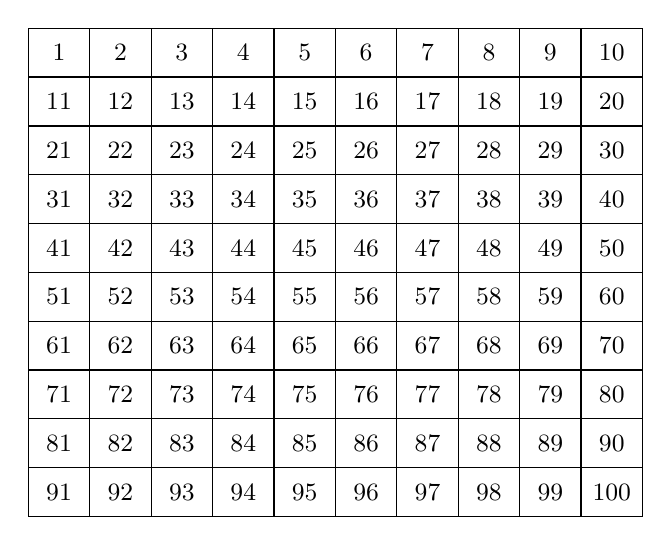
\begin{tikzpicture}[x=0.78cm,y=0.62cm]
  \foreach \n in {1,...,100}{
    \pgfmathtruncatemacro{\col}{mod(\n-1,10)}
    \pgfmathtruncatemacro{\lig}{9-floor((\n-1)/10)}
    \draw[line width=0.45pt] (\col,\lig) rectangle ++(1,1);
    \node[font=\small] at (\col+0.5,\lig+0.5) {\n};
  }
\end{tikzpicture}}

\begin{document}

\titreseq{Activité 3 -- Le crible d'Ératosthène}

\remarque{Le crible permet de retrouver tous les nombres premiers
inférieurs à \(100\) sans tester tous leurs diviseurs un par un.}

\section*{Partie A -- Appliquer l'algorithme}

Sur la grille :

\begin{enumerate}
  \item barre \(1\) ;
  \item entoure \(2\), puis barre tous ses multiples sauf \(2\) ;
  \item entoure le plus petit nombre non barré ;
  \item barre tous ses multiples, sauf lui-même ;
  \item recommence jusqu'à ce que tous les nombres soient
        entourés ou barrés.
\end{enumerate}

\begin{center}
\grillecent
\end{center}

\section*{Partie B -- Comprendre l'algorithme}

\begin{enumerate}
  \item Pourquoi ne barre-t-on pas le nombre que l'on vient d'entourer ?
  \item Lorsqu'on barre un multiple de \(5\), pourquoi sait-on qu'il n'est pas premier ?
  \item Certains nombres sont barrés plusieurs fois.
        Donne un exemple et explique pourquoi.
  \item Que représentent les nombres qui restent entourés ?
\end{enumerate}

\lignesreponse{6}

\section*{Partie C -- Construire la liste à connaître}

Recopie les nombres premiers inférieurs à \(100\), rangés par dizaines.

\renewcommand{\arraystretch}{1.55}
\begin{tabularx}{\textwidth}{
|>{\centering\arraybackslash}p{2.7cm}
|>{\raggedright\arraybackslash}X|}
\hline
\textbf{Intervalle} & \textbf{Nombres premiers}\\
\hline
De \(1\) à \(9\) & \\
\hline
De \(10\) à \(19\) & \\
\hline
De \(20\) à \(29\) & \\
\hline
De \(30\) à \(39\) & \\
\hline
De \(40\) à \(49\) & \\
\hline
De \(50\) à \(59\) & \\
\hline
De \(60\) à \(69\) & \\
\hline
De \(70\) à \(79\) & \\
\hline
De \(80\) à \(89\) & \\
\hline
De \(90\) à \(99\) & \\
\hline
\end{tabularx}

\section*{Partie D -- Premiers ou composés ?}

Pour chaque nombre, indique s'il est premier.
S'il ne l'est pas, écris-le sous la forme d'un produit de deux entiers
strictement supérieurs à \(1\).

\[
51\qquad 53\qquad 57\qquad 67\qquad 77\qquad 83\qquad 91
\]

\lignesreponse{5}

\aretenir{Pour montrer qu'un entier n'est pas premier,
il suffit de trouver un diviseur différent de \(1\) et de lui-même.}

\end{document}
